\scanpage{22}

\handwritten{%
% L1–3 upper left
\[
 \begin{aligned}
 B\quad\underline{B'\amalg B''}\qquad&
 \unsure{\zeta|\xi}_{14}\ \zeta_{15}\ \zeta_{16}\\
 &\zeta_{\unsure{24|23}}\ \zeta_{25}\ \zeta_{\unsure{26|22}}\\
 &\zeta_{24}\ \zeta_{\unsure{25|35}}\ \zeta_{26}
 \end{aligned}
\]

% L2–3 upper left
\figure{
\begin{tikzpicture}[scale=.5]
\foreach \p in {(0,1),(.6,1),(.98,1),(2.25,.94),(.62,.28),(1,.26),(2.27,.24),(3.35,.18)}{\fill \p circle (1.35pt);}
\draw[thick] (1,.26)--(2.27,.24) (2.25,.94)--(3.35,.9);
\end{tikzpicture}}

% L1–5 upper centre
\[
 \begin{array}{r}36\\36\\\hline216\\108\phantom{0}\\\hline1296\\1440\end{array}
 \qquad 
\begin{tikzpicture}[scale=.35]\foreach \y in {0,.45,.9}{\draw (0,\y)--(.85,\y-.5);}\end{tikzpicture}
\]

% L4–5 left
\figure{\begin{tikzpicture}[scale=.45]\foreach \x in {0,.7}{\foreach \y in {0,.55,1.1}{\fill (\x,\y) circle (1.25pt);}}\draw (-.3,.78)--(-.2,-.2);\end{tikzpicture}}

% L5
$\ldots$ trièdres $\longleftrightarrow$ hexagones

% L6–7
\[
 \begin{aligned}
 6^4&=36\mathbin{\unsure{\times|<}}36=2^4\,3^4\\
 720&=\underline{2^{\unsure{4|3}}\cdot3^2}\cdot5.\qquad 9/5
 \end{aligned}
 \qquad
 \left\{\begin{array}{l}40\\\deleted{45}\,36\\45\end{array}\right.
\]

% L8 between horizontal rules
\unsure{Problème|Partons|Partition} \unsure{orbitier|plutôt|ordonnée} d'un \deleted{\unsure{tri}}

% L9
\[
 \zeta_{12}\ \zeta_{23}\ \zeta_{31}\ \big|\ \zeta_{45}\
 \overset{\leftrightarrow}{\check{\zeta}_{56}}\ \zeta_{64}
\]

% L10–14 middle left
\figure{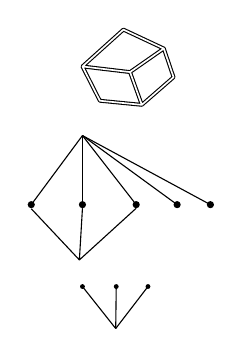
\begin{tikzpicture}[scale=.65,line join=round]
\draw[double] (0,2.7)--(.8,3.42)--(1.59,3.05)--(1.78,2.49)--(1.16,1.95)--(.34,2.03)--cycle (0,2.7)--(.93,2.59)--(1.59,3.05) (.93,2.59)--(1.16,1.95);
\foreach \x in {-1,0,1.05,1.85,2.5}{\draw (0,1.35)--(\x,0);\fill (\x,0) circle (2pt);}
\draw (-1,-.08)--(-.06,-1.08)--(1.05,-.07) (-.06,-1.08)--(0,-.07);
\foreach \x in {0,.66,1.28}{\draw (.65,-2.42)--(\x,-1.6);\fill (\x,-1.6) circle (1.35pt);}
\end{tikzpicture}}

% L10–13 middle right

\begin{tikzpicture}[x=.5cm,y=.5cm]\draw (0,0)--(1,.08)..controls (1.5,-.12) and (2,.1)..(3,.13)--(5,.3)--(6,.26);\foreach \x/\y in {0/0,1/.08,3/.13,4.75/.21,5.15/.17}{\fill (\x,\y) circle (1pt);}\end{tikzpicture}

\unsure{se répartissent} en \unsure{liés au}

$\deleted{\unsure{\zeta}}\zeta_{ij}\qquad \deleted{\unsure{\zeta}}\zeta_{ij}\quad i,j\in\{1,\ldots,6\}$

\unsure{en} \unsure{iBs|i et j} $\longrightarrow$ non liés

% L14 middle right
\[
 \zeta_{12}\ \zeta_{13}\ -\ \zeta_{16}
\]

}
% printed form, rotated 180 degrees, left column
% printed form
N\textsuperscript{o}

UNIVERSITÉ DES SCIENCES\\
ET TECHNIQUES\\
DU LANGUEDOC

(1) -- Le candidat doit indiquer la nature de l'examen auquel il se présente.

(2) -- Le candidat inscrit ses nom, prénom, lieu et date de naissance en tête de la copie et signe lisiblement son nom à la fin de la composition.

% printed form, rotated 180 degrees, main column
% printed form
ACADEMIE DE MONTPELLIER

\textit{Examen de} \textsuperscript{(1)} \dotfill\\
\mbox{}\dotfill

\textit{Nom et Prénoms du Candidat} \textsuperscript{(2)} \dotfill

\textit{né à} \dotfill\quad \textit{département de} \dotfill

\textit{le} \dotfill\quad 19

\textit{Montpellier, le} \dotfill\quad 19

COMPOSITION EN \dotfill
% archive sheet number: 21
